\documentclass[9pt,twocolumn,twoside,]{pnas-new}

%% Some pieces required from the pandoc template
\providecommand{\tightlist}{%
  \setlength{\itemsep}{0pt}\setlength{\parskip}{0pt}}

% Use the lineno option to display guide line numbers if required.
% Note that the use of elements such as single-column equations
% may affect the guide line number alignment.


\usepackage[T1]{fontenc}
\usepackage[utf8]{inputenc}

% For Pandoc highlighting needs

% Pandoc citation processing


\templatetype{pnasresearcharticle}  % Choose template

\title{Identifying Risk Factors Responsible for Differences in Birth
Weight}

\author[a]{Michael Podbury}
\author[a]{Name}

  \affil[a]{The University of Sydney, NSW, 2008}


% Please give the surname of the lead author for the running footer
\leadauthor{Podbury}

% Please add here a significance statement to explain the relevance of your work
\significancestatement{}


\authorcontributions{}



\correspondingauthor{\textsuperscript{} }

% Keywords are not mandatory, but authors are strongly encouraged to provide them. If provided, please include two to five keywords, separated by the pipe symbol, e.g:
 \keywords{  birth weight |  maternal health |  multiple linear
regression  } 

\begin{abstract}
This study is aimed to investigate how the mother's health state
influences the infant birth weight through developing a multiple linear
regression model for prediction. The final model is formulated by
applying the Akaike Information Criterion(AIC) and manually removing
inappropriate predictors based on justifying the significance level.
Results illustrate that the higher mothers' last menstrual weight aided
in the increase in birth weight. However, non-white race, uterine
irritation, smoking, and hypertension can cause a decreasing impact on
birth weight, which is consistent with prior research. The adjusted
r-squared of the final model is 0.195 which reflects that the
goodness-of-fit in the regression model may not be as expected, also
suggesting a limited extent in explaining the total variance of observed
birth weight.
\end{abstract}

\dates{This manuscript was compiled on \today}
\doi{\url{www.pnas.org/cgi/doi/10.1073/pnas.XXXXXXXXXX}}

\begin{document}

% Optional adjustment to line up main text (after abstract) of first page with line numbers, when using both lineno and twocolumn options.
% You should only change this length when you've finalised the article contents.
\verticaladjustment{-2pt}

\maketitle
\thispagestyle{firststyle}
\ifthenelse{\boolean{shortarticle}}{\ifthenelse{\boolean{singlecolumn}}{\abscontentformatted}{\abscontent}}{}

% If your first paragraph (i.e. with the \dropcap) contains a list environment (quote, quotation, theorem, definition, enumerate, itemize...), the line after the list may have some extra indentation. If this is the case, add \parshape=0 to the end of the list environment.

\acknow{}

\hypertarget{introduction}{%
\section*{Introduction}\label{introduction}}
\addcontentsline{toc}{section}{Introduction}

\hypertarget{Background}{%
\subsection*{Background}\label{Background}}
\addcontentsline{toc}{subsection}{Background}

Birth weight is closely related to the newborn's immediate and long term
health. Low birth weight (\textless{} 2500 grams) babies may be more
prone to certain health issues, such as sickness or infection even death
in infancy, as well as susceptibility to chronic diseases later in life.
High birth weight (\textgreater4000 grams) is also linked to an
increased risk of birth injuries, infancy mortality and long-term
secretion disorders. In summary, birth weight is strongly associated
with a range of health outcomes. Therefore, the medical profession and
society have been widely concerned for decades about the management of
birth weight, and researches indicates that infant birth weight is
hugely influenced by modifiable maternal pre-pregnancy health behaviors
and characteristics.For instance, birth weight has innate racial
disparities and is positively associated with the maternal level of
obesity or emaciation before pregnancy. Additional, smoking during
pregnancy and tobacco exposure have been shown to significantly reduce
the weight of newborns; advanced (\textgreater35 yr) or low (\textless16
yr) maternal age, and women with history of hypertension or uterine
irritability, are also more likely to deliver infants with a lower
weight. Also, inadequate prenatal care can further raise the probability
of premature labor and aberrant birth weights. The purpose of this study
is to build a multiple linear regression model to predict newborn's
birth weight given maternal health condition, in order to explore the
answer of question that which factors have a substantial or weak impact
on infant birth weight.

\hypertarget{data-set}{%
\subsection*{Data Set}\label{data-set}}
\addcontentsline{toc}{subsection}{Data Set}

The \emph{birthwt} data set is sourced from Baystate Medical Center in
1986. However, the details of who collected the data and what was the
method of collection are unclear. It contains 189 observations of birth
and 10 variables, two of them are related to the baby's
\emph{birth\_weight} (dependent variable), while the other eight
variables are the records about maternal health and behavior conditions.
Data cleaning includes: attributes are renamed for readability; discrete
counts are transformed into factors; binary indicators are converted
into Boolean values (True or False). For the only two
\textbf{quantitative} independent variables: mother's \emph{age} and her
weight in pounds at last menstrual period,
\emph{weight\_last\_menstrual}, the outliers are removed to improve the
statistical power. The remaining qualitative variables includes: race,
which has three groups, white for 0, black for 1 and other for 3; the
\emph{smoking\_status}, whether the mother smoking during pregnancy;
whether she has a history of \emph{hypertension}; \emph{uterine\_irr},
whether she has presence of uterine irritability. Besides, the number of
premature labour counts, as \emph{premature\_labor} is categorized into
binary group, 0 or 1+; the number of physician visits during the first
trimester, as \emph{physician\_visits} is factorized into three groups,
0, 1, or 2+. Since the spread of these two variables are not widely and
evenly enough, combine categories with extremely few observations to
avoid being limited by the insufficient quantity.

\hypertarget{analysis}{%
\section*{Analysis}\label{analysis}}
\addcontentsline{toc}{section}{Analysis}

\hypertarget{assumptions}{%
\subsection*{Assumptions}\label{assumptions}}
\addcontentsline{toc}{subsection}{Assumptions}

To guarantee the validity, the assumption checks were performed both
before and after variable selection, that is, both for full model and
final model. First, continuous data that do not fit the linearity
assumption should be removed, such as the age variable, which the
attempt of Log transformation still unable to satisfy the linear
relationship with the dependent variable. Furthermore, Log transform the
\emph{birth\_weight} can strengthen the linear relationship between it
and the \emph{weight\_last\_mentrual} variable. Thus, the Log transfer
of the dependent variable (\emph{birth\_weight}) will be retained in the
following study. Second, Categorical data that does not meet the
assumptions of equal variance across groups or normal distribution
should be removed as well. However, following data preprocessing, the
remaining qualitative variables all satisfy this assumption. In
addition, since each mother is autonomous, the health status or
behaviors of one should not affected by the other, the independence
assumption is justified. Third, the residual plot of final model shows
that the residuals' spread is almost symmetrically distributed, tending
to cluster towards the middle of the plot and not has a clear patterns.
It represents the dispersion of the residual is consistent across the
range of fitted birth\_weight values, so that satisfy with the
homoskedasiticity assumption. Eventually, the residual qq plot
demonstrates that most of the points closely follow to the 45-degree
line, very less or negligible deviation at the ends, also relating on
the CLT(Central Limit Theorem) thus the normality can be assumed.

\begin{figure}[h]
\centering

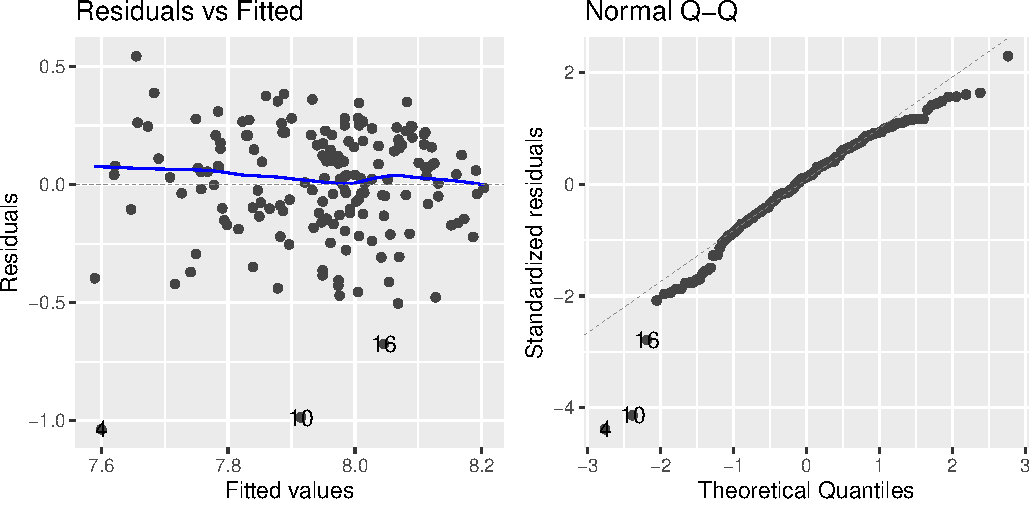
\includegraphics[width=240px,height=150px]{report_files/figure-latex/unnamed-chunk-1-1} 
\caption{Residuals plots for the final regression model}
\end{figure}

\hypertarget{model-selection}{%
\subsection*{Model Selection}\label{model-selection}}
\addcontentsline{toc}{subsection}{Model Selection}

Because the \emph{age} variable could not be properly addressed the
linearity assumption regardless of whether the log transformation was
applied or not, it was eliminated completely.The parameter selection of
final model is determined by the forward and backward stepwize Akaike
information criterion (AIC). Variables are added to the null model in
the forward method and removed from the full model in the backward
method, until the AIC no longer decreased, so that develop the model
with a section of predictors that performed AIC value as low as
possible. And it shows that bot method excluded the age variable which
doesn't fit the regression assumption. However, the p-value of
\emph{smoking\_status} variable (0.053) is greater than the significance
level(0.05), which indicates that whether or not the mother smokes has
no significant influence on the birth weight, so the
\emph{smoking\_status} predictor is decided to be manually removed from
the final model. Moreover, though the p-value of
\emph{weight\_last\_menstrual} represents it significantly impact the
dependent variable, the value of estimates, in terms of the beta
multiplier in front of the predictor is 0, which indicates the variable
has no mathematical meaning for predicting results. These contradict the
findings of several previous researches. This contradiction might be due
to the log transformation of dependent variable, insufficient sample
size or selection bias generated by the single source (only one medical
center) of observation, or other potential cause that can be improved in
the further research.

\hypertarget{results}{%
\section*{Results}\label{results}}
\addcontentsline{toc}{section}{Results}

\hypertarget{inferences}{%
\subsection*{Inferences}\label{inferences}}
\addcontentsline{toc}{subsection}{Inferences}

\[\begin{aligned}
\operatorname{log(birth\_weight)}=&7.8442-0.1314(\operatorname{race}_{\operatorname{black}})
                             -0.1152(\operatorname{race}_{\operatorname{other}})\\
                             &+0.0020(\operatorname{last\_menstrual\_weight})\\
                             &-0.2143(\operatorname{uterine\_irritability}_{\operatorname{TRUE}}) \\
                             &-0.2679(\operatorname{hypertension}_{\operatorname{TRUE}}) \\
                             &-0.1020(\operatorname{smoke}_{\operatorname{TRUE}})+\epsilon
\end{aligned} \]

As the formula suggests, when all other conditions stay consistent,
racial background other than black can contribute to a larger baby.'

Explain the coefficients.

\hypertarget{performance}{%
\subsection*{Performance}\label{performance}}
\addcontentsline{toc}{subsection}{Performance}

We compared our final model with the full model which contains all
variables in the data set being used as predictors. Out of sample
performances are tested using ``Caret'' package at a 10-fold
cross-validation.

How good is your model?

\begin{table}[h]
\caption{Performance results of models}
\centering
\begin{tabular}{|l|l|l|l|}
\hline
\textbf{Attributes} & \textbf{Full Model} & \textbf{Final Model} \\ \hline
adjusted r-squared & 0.2291 & 0.2154 \\ \hline
In Sample RMSE & 612.5661 & 633.8657 \\ \hline
In Sample MAE & 494.3237 & 513.9027 \\ \hline
Out of Sample RMSE & 664.8032 & 655.9306 \\ \hline
Out of Sample MAE & 543.8441 & 533.437 \\ \hline
Out of Sample r-squared & 0.1927145 & 0.2239073 \\ \hline
\end{tabular}
\end{table}

\hypertarget{discussion}{%
\section*{Discussion}\label{discussion}}
\addcontentsline{toc}{section}{Discussion}

\hypertarget{limitations}{%
\subsection*{Limitations}\label{limitations}}
\addcontentsline{toc}{subsection}{Limitations}

In general: The low adjusted r-squared value 0.195 indicates that the
final model only able to explain 19.5\% of total birth weight variance.
The reliability of model is questionable since sample size is small (189
observations),which has limited the ability to predict infant birth
weight by five predictors. Therefore, a larger set would have preferred
to increase the reliability of model. The data was collected in 1986
which is outdated, the demography is very likely to have changed
significantly,so the condition may be inconsistent with the
present.Better medical treatment, social welfare, and human rights
equality have evened out elements such as racial origin in terms of how
they contribute to birth weight. All observations are form only one
medical center may cause the lack of sample diversity. As a result of
the selection bias, our model is incapable of effectively capturing the
whole human population.

There is no information about who and how the data is collected, so the
accuracy and credibility of the data are in doubt.It may cause
measurement bias due to improper data collection method.

For specific variables: Only 12 of the 189 women had a history of
hypertension, making it difficult to determine if birth weight is
normally distributed for this group, and there will be deviations owing
to insufficient sample size when measuring the influence of this
variable.

It only notes whether the mother smokes, but it does not specify how
long she has smoked, how frequently she smokes, or whether she has other
tobacco-related habits that may impact her birth weight.

Just the mother's weight without height may be insufficient to
adequately depict the mother's health. The body mass index will help
better understand the link between the mother maternal weight and the
baby's weight.

Moreover, additional factors that have been discovered to have a
significant impact on birth weight in previous research, such as the
baby's gestational age, indicator of gestational diabetes and average
alcohol intake during the duration of the pregnancy are not addressed
by.The inadequate consideration of potential factors may also reduce the
predictive power of the final model.

\hypertarget{conclusion}{%
\subsection*{Conclusion}\label{conclusion}}
\addcontentsline{toc}{subsection}{Conclusion}

Future investigations should xxx.

Nevertheless, the analysis of the data gives us a glimpse of some
lifestyle factors parents may look out for to have children with a
healthy birth weight. \ldots{}

\hypertarget{references}{%
\section*{References}\label{references}}
\addcontentsline{toc}{section}{References}

\href{https://github.sydney.edu.au/}{GitHub repository}

{[}1{]} Bernstein, I., Mongeon, J., Badger, G., Solomon, L., Heil, S.
and Higgins, S., 2005. Maternal Smoking and Its Association With Birth
Weight. Obstetrics \& Gynecology, 106(5, Part 1), pp.986-991.

{[}2{]} England, L., 2001. Measures of Maternal Tobacco Exposure and
Infant Birth Weight at Term. American Journal of Epidemiology, 153(10),
pp.954-960.

{[}3{]} Frederick, I., Williams, M., Sales, A., Martin, D. and Killien,
M., 2007. Pre-pregnancy Body Mass Index, Gestational Weight Gain, and
Other Maternal Characteristics in Relation to Infant Birth Weight.
Maternal and Child Health Journal, 12(5), pp.557-567.

{[}4{]} Goisis, A., Remes, H., Barclay, K., Martikainen, P. and
Myrskylä, M., 2017. Advanced Maternal Age and the Risk of Low Birth
Weight and Preterm Delivery: a Within-Family Analysis Using Finnish
Population Registers. American Journal of Epidemiology, 186(11),
pp.1219-1226.

{[}5{]} González-Jiménez, J., \& Rocha-Buelvas, A. (2018). Risk factors
associated with low birth weight in the Americas: literature review.
Revista De La Facultad De Medicina, 66(2), 255-260. doi:
10.15446/revfacmed.v66n2.61577

{[}6{]} Journal of Nurse-Midwifery, 1986. Maternal weight and birth
weight Abrams B, Laros R: Prepregnancy weight, weight gain, and birth
weight. AM 3 OBSTET GYNECOL 154:503, 1986. 31(5), p.242.

{[}7{]} Rahfiludin, M., \& Dharmawan, Y. (2018). Risk Factors Associated
with Low Birth Weight. Kesmas: National Public Health Journal, 13(2).
doi: 10.21109/kesmas.v13i2.1719

{[}8{]} (2021). Retrieved 27 October 2021, from
\url{https://www.who.int/classifications/icd/ICD-10_2nd_ed_volume2.pdf}

{[}9{]} Wilcox, A., 2001. On the importance---and the unimportance--- of
birthweight. International Journal of Epidemiology, 30(6), pp.1233-1241.

{[}10{]} Wiley-Blackwell. (2011, December 13). Mothers' weight before
and during pregnancy affects baby's weight. ScienceDaily. Retrieved
October 25, 2021 from
www.sciencedaily.com/releases/2011/12/111213110521.htm

\showmatmethods
\pnasbreak



% Bibliography
% \bibliography{pnas-sample}

\end{document}
